\documentclass[12pt,a4paper]{article}
\usepackage[utf8]{inputenc}
\usepackage[russian]{babel}
\usepackage[OT1]{fontenc}
\usepackage{mathtools}
\usepackage{amsfonts}
\usepackage{amssymb}
\usepackage{enumitem}
\usepackage{alltt}
\usepackage{graphicx}
\usepackage{indentfirst}
\usepackage{caption}
\usepackage{float}
\usepackage{wrapfig}
\usepackage{physics}
\usepackage{multirow}
\usepackage{longtable}
\usepackage{amsmath,amsfonts,amssymb,amsthm,mathtools}
\usepackage{icomma}
\setlength{\parindent}{0.75cm}
\graphicspath{{pictures/}}
\DeclareGraphicsExtensions{.png, .jpg}
\usepackage[left=15mm,right=15mm,top=2cm,bottom=2cm]{geometry}
\author{Глотов Алексей}
\begin{document}
\newpage
\begin{center}
\footnotesize{{ГОСУДАРСТВЕННОЕ АВТОНОМНОЕ ОБРАЗОВАТЕЛЬНОЕ УЧРЕЖДЕНИЕ}\break
{ВЫСШЕГО ОБРАЗОВАНИЯ}
\break
{\bf {МОСКОВСКИЙ ФИЗИКО-ТЕХНИЧЕСКИЙ ИНСТИТУТ}}
\break
\small{(НАЦИОНАЛЬНЫЙ ИССЛЕДОВАТЕЛЬСКИЙ УНИВЕРСИТЕТ)}}
\break
\hfill \break
\hfill \break
\begin{center}
\normalsize{Кафедра общей физики}
\end{center}
\hfill \break
\hfill \break
\hfill \break
\hfill \break

\begin{center}
\normalsize {Лабораторная работа 5.4.2}
\end{center}
\hfill \break\\
\large{\textbf{Исследование энергетического спектра бета-частиц и определение их максимальной энергии при помощи магнитного спектрометра}}
\end{center}
\begin{flushleft}
\hfill \break
\hfill \break
\hfill \break
\hfill \break
\hfill \break
\hfill \break
\hfill \break
\hfill \break
\hfill \break
\hfill \break
\hangindent=10cm
\normalsize{Преподаватель:} \;\;\;\;
\normalsize{к.ф.-м.н. Юрьев Ю.В.}\\
\hfill \break
\normalsize{Обучающийся:} \;\;\;\;\;
\normalsize{Глотов А.А} \\
\hfill \break
\end{flushleft}
\hfill \break
\hfill \break
\hfill \break
\hfill \break
\hfill \break
\hfill \break
\hfill \break
\hfill \break
\hfill \break
\hfill \break
\hfill \break

\begin{center}
Долгопрудный \break
 2023
\end{center}

\thispagestyle{empty}


\newpage
\section{Введение}

\subsection{Аннотация}

	Бета - распадом называется самопроизвольное превращение ядер, при котором их массовое число не меняется, а заряд увеличивается или уменьшается на единицу. Бета распад является внутренуклонным процессом, например, при $\beta^-$ распаде нейтрон распадается на протон, электрон и электронное антинейтрино. В нашей работе мы будем иметь дело именно с таким типом распада:

\begin{equation}
^A_Z X -> ^A_{Z+1} X + e^- + \tilde{\nu}
\end{equation}	

Цель: исследовать энергетический спектр бета-частиц при распаде ядер ($_55^137$)Cs, определить их максимальную энергию.


\subsection{Теоретические сведения}
Результатом бета-распада, помимо вылета электрона, является также вылет антинейтрино. Почти вся энергия, выделяющаяся в ходе данного процесса, оказывается разделённой между этими двумя частицами, поэтому выполняется:
\begin{equation}
T_{max} - T_e - E_\nu=0
\end{equation}
Здесь $T_max$ – максимально возможная в данном распаде кинетическая энергия электрона, $T_e$ – его фактическая кинетическая энергия, $E_\nu$ – энергия антинейтрино.

	Величиной W($p_e$)d$p_e$ назовём вероятность того, что электрон получит при испускании импульс, лежащий в интервале ($p_e$; $p_e$+d$p_e$ ).
Имеем:
\begin{equation}
W(p_e)dp_e \varpropto p_e^2 (T_{max} - T_e )^2 dp_e
\end{equation}

	Исходя из этого выражения, можно видеть, что зависимость W($p_e$) имеет вид колокола.

	Дочерние ядра, образующиеся при бета-распаде, часто оказываются в возбуждённом состоянии, они отдают свою энергию либо испуская гамма квант, либо передавая избыток энергии одному из электронов. Излучаемые в таком процессе электроны имеют строго определённую энергию и называются конверсионными. В результате конверсии в спектре появляется монохроматическая линия, ширина которой обуславливается только лишь неточностью аппаратуры. По ней можно определить разрешающую силу спектрометра.

\begin{figure}[h]
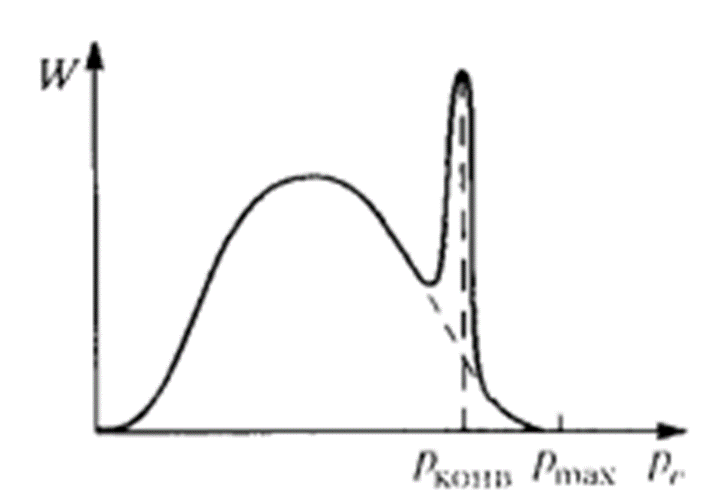
\includegraphics[scale = 0.5]{5.4.2-1}
\centering
\caption{Вид энергетического спектра бета-распада}
\end{figure}


\subsection{Экспериментальная установка}

Основным элементом установки является магнитная линза (катушка), по сути являющаяся аналогом обычной линзы для заряженных частиц. Её фокусное расстояние зависит от импульса электрона и индукции магнитного поля (т.е. силы тока в катушке) следующим образом:

\begin{center}
$\frac{1}{l} \pitchfork \frac{I^2}{p_e^2}$
\end{center}

При неизменной силе тока, на счётчик будут попадать электроны с определённым импульсом, другие же будут проходить мимо. 

\begin{figure}[h]
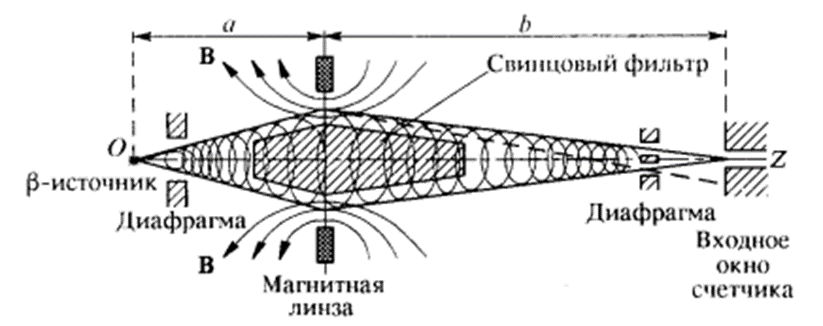
\includegraphics[scale = 0.7]{5.4.2-2}
\centering
\caption{Cхема бета-спектрометра}
\end{figure}

     Из-за конечных размеров источника, диафрагм, ограничивающих углы вылета, и окна счётчика, а также в следствие аберраций, при заданной величине тока в катушке, на счётчик попадают электроны имеющий импульс, лежащий в промежутке ($p_e$-$\frac{\Delta p_e}{2} ; p_e + (\frac{\Delta p_e}/{2})$. Величина $\Delta p_e$ называется разрешающей способностью спектрометра. Разрешающая способность также зависит и от диаметра свинцового фильтра, необходимого для отсеивания электронов, летящих по центру, на траекторию которых не способно повлиять магнитное поле. 
     Число частиц, регистрируемых установкой, связано с W следующим образом:
     \begin{equation}  
N(p_e )=CW(p_e ) p_e
     \end{equation}
Где C – некоторая константа, определяемая геометрией установки.

     С помощью форвакуумного насоса давление внутри спектрометра уменьшают до 0,1 Тор. Это сделано для того, чтобы вещество внутри не мешало прохождению электронов. 


\begin{figure}[h]
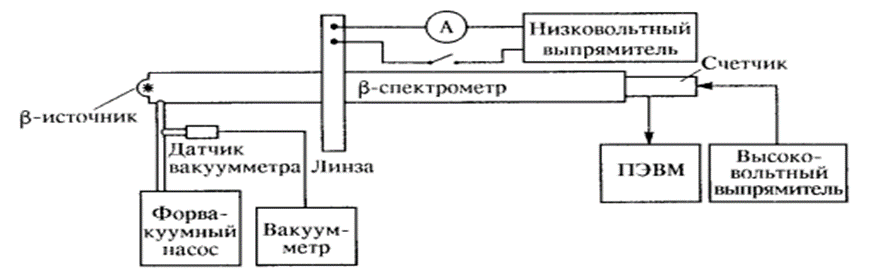
\includegraphics[scale = 0.7]{5.4.2-3}
\centering
\caption{Схема установки}
\end{figure}

\section{Результаты измерений и обработка данных}

     Для различных значений тока компьютерная программа может посчитать, число электронов в единицу времени, которое попадает на счётчик. Зная, что произведение импульса конверсионного электрона на скорость света равно 1013,5 КэВ произведём пересчёт от тока к импульсу. Аналогично можно произвести пересчёт к энергии, зная, что энергия внутренней конверсии равна 634 КэВ. Учитывая фон, по этим данным построим таблицу: (время измерения составляет t=100 с).
     
     \begin{center} \begin{Large}
\begin{tabular}{|c|c|c|c|c|}
     \hline 
     № & I, А & N - $N_\text{ф}$, с$^{-1}$ & T, кэВ & p, кэВ/c \\ 
     \hline 
     1 & 0,00 & -0,015 & 0,0 & 0,0 \\ 
     \hline 
     2 & 0,2 & 0,065 & 2,4 & 49,7 \\ 
     \hline 
     3 & 0,4 & 0,095 & 9,6 & 99,4 \\ 
     \hline 
     4 & 0,60 & 0,105 & 21,3 & 149,1 \\ 
     \hline 
     5 & 0,8 & 0,405 & 37,3 & 198,9 \\ 
     \hline 
     6 & 1,00 & 0,765 & 57,2 & 248,6 \\ 
     \hline 
     7 & 1,20 & 1,364 & 80,7 & 298,3 \\ 
     \hline 
     8 & 1,40 & 1,994 & 107,2 & 348,0 \\ 
     \hline 
     9 & 1,60 & 2,264 & 136,5 & 397,7 \\ 
     \hline 
     10 & 1,80 & 3,314 & 168,2 & 447,4 \\ 
     \hline 
     11 & 2,00 & 3,894 & 201,9 & 497,1 \\ 
     \hline 
     12 & 2,20 & 3,454 & 237,4 & 546,9 \\ 
     \hline 
     13 & 2,40 & 4,133 & 274,5 & 596,6 \\ 
     \hline 
     14 & 2,60 & 4,143 & 312,9 & 646,3 \\ 
     \hline 
     15 & 2,80 & 3,444 & 352,4 & 696,0 \\ 
     \hline 
     16 & 3,00 & 3,024 & 393,0 & 754,7 \\ 
     \hline 
     17 & 3,20 & 1,984 & 434,4 & 795,4 \\ 
     \hline 
     18 & 3,40 & 1,264 & 476,6 & 845,1 \\ 
     \hline 
     19 & 3,60 & 0,635 & 519,5 & 894,9 \\ 
     \hline 
     20 & 3,80 & 0,964 & 562,9 & 944,6 \\ 
     \hline 
     21 & 3,90 & 2,724 & 584,9 & 969,4 \\ 
     \hline 
     22 & 4,00 & 3,944 & 606,9 & 994,3 \\ 
     \hline 
     23 & 4,10 & 5,763 & 629,1 & 1019,1 \\ 
     \hline 
     24 & 4,20 & 5,143 & 651,3 & 1044,0 \\ 
     \hline 
     25 & 4,30 & 4,064 & 673,7 & 1068,9 \\ 
     \hline 
     26 & 4,40 & 1,164 & 696,2 & 1093,7 \\ 
     \hline 
     \end{tabular}      
     \end{Large}
     \end{center}

Здесь погрешность измерений : I $\pm 0.01$ A, (N - $N_\text{ф}$) $\pm \sqrt{N / 100}$, T $\pm 0.1$ кэВ, p $\pm$ 0.1 кэВ/с.   

По этим данным построим график зависимости N - $N_\text{ф}$=f(p)

\begin{figure}[H]
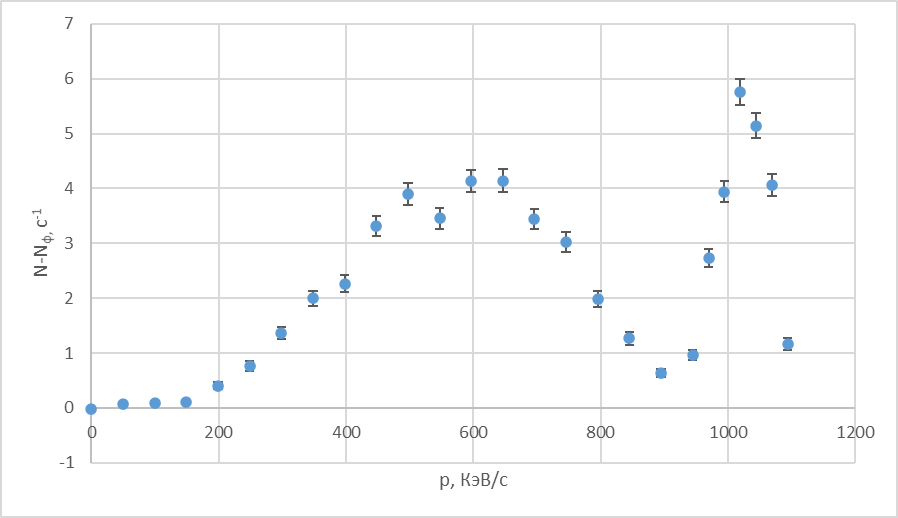
\includegraphics[scale = 0.7]{5.4.2-4}
\centering
\end{figure}

	Построим график Ферми-Кюри. По оси абсцисс будем откладывать энергию, а по оси ординат величину $\frac{\sqrt(N - N_\text{ф})(p)}{p^{3/2}}$ . Из соотношений, приведённых в теоретических сведениях, можно получить, что выполнено следующее:
\begin{center}
$\frac{\sqrt(N - N_\text{ф})(p)}{p^{3/2}}$ = $T_{max}$ - T
\end{center}	

 Так график будет иметь отрицательный угол наклона и пересекать ось абсцисс в точке максимальной энергии бета-распада.
     
   \begin{figure}[H]
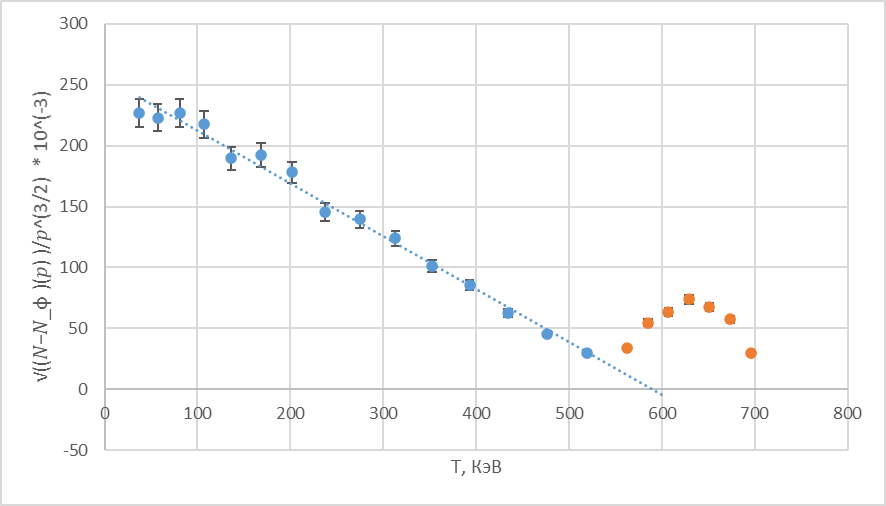
\includegraphics[scale = 0.7]{5.4.2-5}
\centering
\end{figure}  

Используя линейную аппроксимацию по МНК получаем, что максимальная кинетическая энергия бета-распада равна:
\begin{center}
$T_{max}$ = (590 $\pm$ 30) кэВ
\end{center}

\end{document}